\documentclass[uplatex, 12pt, dvipdfmx]{jsarticle}
\title{ことば}
\author{司馬 博文}
\date{\today}
\pagestyle{empty} \setcounter{secnumdepth}{4}
\input{/Users/Hirofumi Shiba/NatureOfStatistics/preamble_no_fonts.tex}
%\input{/Users/hirofumi.shiba48/NatureOfStatistics/preamble_no_fonts.tex}

\newcommand{\egg}[1]{\raisebox{-3pt}{
\begin{tikzpicture}[x=1pt,y=1pt,line width=1pt]
\draw (0,0) ellipse (4.5 and 6);
\draw (0,0) node {\fontfamily{phv}\fontsize{9pt}{0}\selectfont #1\/};
\end{tikzpicture}
}}

\renewcommand{\keytop}[2][12]{%
\begin{tikzpicture}[x=0.1em,y=0.1em]
\useasboundingbox (0,0) rectangle (#1,9);
\shadedraw[top color=black!20, rounded corners=0.2em] (0,-3) rectangle (#1,9);
\draw[anchor=base] (#1/2,0) node {\sffamily #2};
\end{tikzpicture}
}

\usetikzlibrary{positioning,automata}

\begin{document}

あ
\tikz\draw(0,0)--(1,2)--(2,0)--(3,2)--(4,0);
\tikz{\draw(0,0)--(10pt,10pt);\draw(0,10pt)--(10pt,0);}

\begin{tikzpicture}
    \draw[step=1,gray] (-0.2,-0.2) grid (2.2,2.2);
    \draw (0.5,0.5) circle (0.5) node {$\pi r^2$};
    \draw[line width=1pt] (1,0) rectangle (2,0.5);
    \fill[black!20] (1,1.5) ellipse (1 and 0.5);
    \draw (1,1.5) node {\hbox{\tate 楕円}};
\end{tikzpicture}

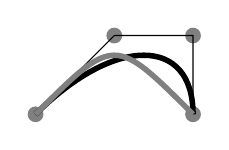
\begin{tikzpicture}[x=1mm,y=1mm]
    \fill[gray] (0,0) circle (1) (10,10) circle (1) (20,10) circle (1) (20,0) circle (1);
    \draw (0,0) -- (10,10) -- (20,10) -- (20,0);
    \draw[line width=2pt] (0,0) .. controls (10,10) and (20,10) .. (20,0);
    \draw[line width=2pt, gray] (0,0) .. controls (10,10) .. (20,0);
\end{tikzpicture}

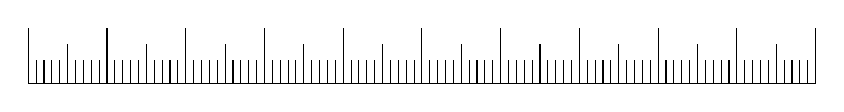
\begin{tikzpicture}[x=1mm,y=1mm]
    \draw (0,0) -- (100,0);
    \foreach \x in {0,...,100} \draw (\x,0) -- (\x,3);
    \foreach \x in {0,5,...,100} \draw (\x,0) -- (\x,5);
    \foreach \x in {0,10,...,100} \draw (\x,0) -- (\x,7);
\end{tikzpicture}

あい\egg{0}うえお

かき\keytop{A}くけこ

\begin{tikzpicture}[>=stealth]
    \draw[->] (-0.5,0) -- (4.2,0) node[right] {$x$};
    \draw[->] (0,-0.5) -- (0,2.2) node[above] {$y$};
    \draw plot[domain=0:4, samples=200] (\x, {sqrt(\x)}) node[below] {$y=\sqrt{x}$};
    \draw (0,0) node[below left] {O};
\end{tikzpicture}

\begin{center}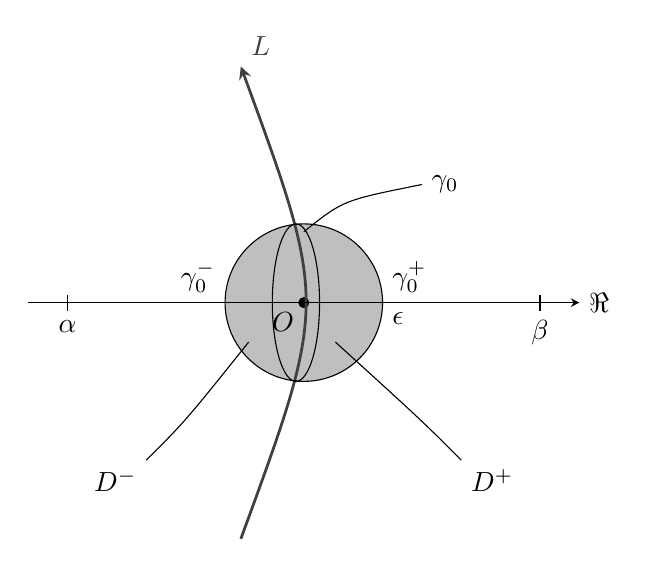
\begin{tikzpicture}[>=stealth]
    \fill[lightgray] (0,0) circle (1);
    \fill[black] (0,0) circle (2pt) node[below left] {$O$};
    \draw[->, line width=1pt, darkgray] (-0.8,-3) .. controls (0.3,0) .. (-0.8,3) node[above right] {$L$};
    \draw[->] (-3.5,0) -- (3.5,0) node[right] {$\Re$};
    \draw (-3,0.1) -- (-3,-0.1) node[below] {$\alpha$};
    \draw (3,0.1) -- (3,-0.1) node[below] {$\beta$};
    \draw (0,0) circle (1);
    \node at (1,0) {\footnotesize$\blacktriangle$};
    \node at (-1,-0.03) {\footnotesize\rotatebox{180}{$\blacktriangle$}};
    \node[below right] at (1,0) {$\epsilon$};
    \node[above right] at (1,0) {$\gamma_0^+$};
    \node[above left] at (-1,0) {$\gamma_0^-$};
    \draw (-0.7,-0.5) .. controls (-1.5,-1.5) .. (-2,-2) node[below left] {$D^-$};
    \draw (0.4,-0.5) .. controls (1.5,-1.5) .. (2,-2) node[below right] {$D^+$};
    \draw (-0.1,0) ellipse (0.3 and 1);
    \draw (0,0.9) .. controls (0.5,1.3) .. (1.5,1.5) node[right] {$\gamma_0$};
\end{tikzpicture}\end{center}

\begin{center}
    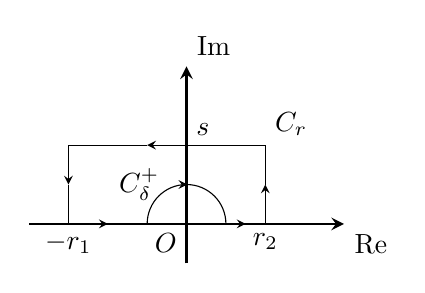
\begin{tikzpicture}[>=stealth]
        \draw[->,line width=1pt] (-2,0) -- (2,0) node[below right] {Re};
        \draw[->,line width=1pt] (0,-0.5) -- (0,2) node[above right] {Im};
        \node[below left] at (0,0) {$O$};
        \draw[->] (1,0) -- (1,0.5);
        \draw (1,0.5) -- (1,1);
        \draw[->] (1,1) -- (-0.5,1);
        \draw (-0.5,1) -- (-1.5,1);
        \draw[->] (-1.5,1) -- (-1.5,0.5);
        \draw (-1.5,0.5) -- (-1.5,0);
        \node[below] at (1,0) {$r_2$};
        \node[below] at (-1.5,0) {$-r_1$};
        \node[above right] at (0,1) {$s$};
        \draw[->] (-1.5,0) -- (-1,0);
        \node[above right] at (1.0,1.0) {$C_r$};
        \draw (0.5,0) arc [radius=0.5, start angle = 0, end angle=180];
        \draw[->] (-0.01,0.5) -- (0.01,0.5);
        \draw[->] (0.5,0) -- (0.75,0);
        \node at (-0.6,0.5) {$C^+_\delta$};
    \end{tikzpicture}
\end{center}

\begin{center}
    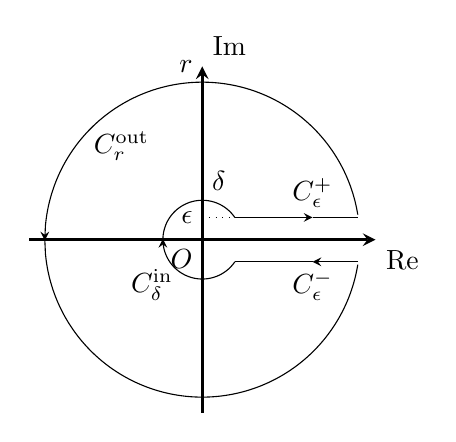
\begin{tikzpicture}[>=stealth]
        \draw[->,line width=1pt] (-2.2,0) -- (2.2,0) node[below right] {Re};
        \draw[->,line width=1pt] (0,-2.2) -- (0,2.2) node[above right] {Im};
        \node[below left] at (0,0) {$O$};
        \draw[domain=-2:1.98, samples=500] plot(\x, {sqrt(4-(\x)^2)});
        \draw[domain=-2:1.98, samples=500] plot(\x, -{sqrt(4-(\x)^2)});
        \draw[domain=-0.5:0.414, samples=500] plot(\x, {sqrt(0.25-(\x)^2)});
        \draw[domain=-0.5:0.414, samples=500] plot(\x, -{sqrt(0.25-(\x)^2)});
        \draw[->] (-0.5,-0.01) -- (-0.5,0.01);
        \draw[->] (-2,0.01) -- (-2,-0.01);
        \draw[->] (0.414,0.282) -- (1.4,0.282);
        \draw (1.4,0.282) -- (1.98,0.282);
        \draw[->] (1.98,-0.282) -- (1.4,-0.282);
        \draw (1.4,-0.282) -- (0.414,-0.282);
        \node[above right] at (0,0.5) {$\delta$};
        \node[above left] at (0,2) {$r$};
        \node[left] at (0,0.282) {$\epsilon$};
        \draw[dotted] (0,0.282) -- (0.414,0.282);
        \node[above] at (1.4,0.282) {$C^+_\epsilon$};
        \node[below] at (1.4,0-.282) {$C^-_\epsilon$};
        \node[below left] at (-0.25,-0.25) {$C_\delta^{\mathrm{in}}$};
        \node[below right] at (-1.5,1.5) {$C_r^{\mathrm{out}}$};
    \end{tikzpicture}
\end{center}

\begin{center}
    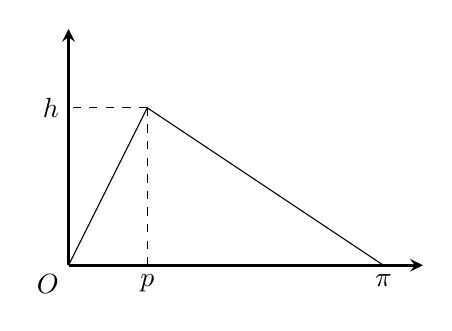
\begin{tikzpicture}[>=stealth]
        \draw[->,line width=1pt] (0,0) -- (4.5,0);
        \draw[->,line width=1pt] (0,0) -- (0,3);
        \node[below left] at (0,0) {$O$};
        \draw[dashed] (1,2) -- (0,2) node[left] {$h$};
        \draw[dashed] (1,2) -- (1,0) node[below] {$p$};
        \draw (0,0) -- (1,2) -- (4,0) node[below] {$\pi$};
    \end{tikzpicture}
\end{center}

\begin{tikzpicture}[>=stealth,x=7mm,y=7mm]
    \node at (0,0) {$\times$};
    \node[below] at (0,0) {$(x_0,y_0)$};
    \draw (-2,-2) -- (2,-2) -- (2,2) -- (-2,2) -- (-2,-2);
    \node[left] at (-2,0) {$h$};
    \node[above] at (0,2) {$h$};
    \draw[->] (2,0) -- (3,0);
    \node[above right] at (2,0) {$(x_0+h/2,y_0)$};
    \node[above left] at (-2,2) {$S$};
\end{tikzpicture}

\end{document}